%%%%%%%%%%%%%%%%%%%%%%%%%%%%%%%%%%%%%%%%%
% Jacobs Landscape Poster
% LaTeX Template
% Version 1.0 (29/03/13)
%
% Created by:
% Computational Physics and Biophysics Group, Jacobs University
% https://teamwork.jacobs-university.de:8443/confluence/display/CoPandBiG/LaTeX+Poster
% 
% Further modified by:
% Nathaniel Johnston (nathaniel@njohnston.ca)
%
% This template has been downloaded from:
% http://www.LaTeXTemplates.com
%
% License:
% CC BY-NC-SA 3.0 (http://creativecommons.org/licenses/by-nc-sa/3.0/)
%
%%%%%%%%%%%%%%%%%%%%%%%%%%%%%%%%%%%%%%%%%

%----------------------------------------------------------------------------------------
%	PACKAGES AND OTHER DOCUMENT CONFIGURATIONS
%----------------------------------------------------------------------------------------

\documentclass[final]{beamer}

\usepackage[scale=1.24]{beamerposter} % Use the beamerposter package for laying out the poster

\usetheme{confposter} % Use the confposter theme supplied with this template

\setbeamercolor{block title}{fg=ngreen,bg=white} % Colors of the block titles
\setbeamercolor{block body}{fg=black,bg=white} % Colors of the body of blocks
\setbeamercolor{block alerted title}{fg=white,bg=dblue!70} % Colors of the highlighted block titles
\setbeamercolor{block alerted body}{fg=black,bg=dblue!10} % Colors of the body of highlighted blocks
% Many more colors are available for use in beamerthemeconfposter.sty

%-----------------------------------------------------------
% Define the column widths and overall poster size
% To set effective sepwid, onecolwid and twocolwid values, first choose how many columns you want and how much separation you want between columns
% In this template, the separation width chosen is 0.024 of the paper width and a 4-column layout
% onecolwid should therefore be (1-(# of columns+1)*sepwid)/# of columns e.g. (1-(4+1)*0.024)/4 = 0.22
% Set twocolwid to be (2*onecolwid)+sepwid = 0.464
% Set threecolwid to be (3*onecolwid)+2*sepwid = 0.708

\newlength{\sepwid}
\newlength{\onecolwid}
\newlength{\onepointfivecolwid}
\newlength{\twocolwid}
\newlength{\threecolwid}
\setlength{\paperwidth}{46.81in} % A0 width: 46.8in
\setlength{\paperheight}{33.11in} % A0 height: 33.1in
\setlength{\sepwid}{0.02\paperwidth} % Separation width (white space) between columns
\setlength{\onecolwid}{0.22\paperwidth} % Width of one column
\setlength{\onepointfivecolwid}{0.33\paperwidth}
\setlength{\twocolwid}{0.464\paperwidth} % Width of two columns
\setlength{\threecolwid}{0.708\paperwidth} % Width of three columns
\setlength{\topmargin}{-0.5in} % Reduce the top margin size
%-----------------------------------------------------------

\usepackage{graphicx}  % Required for including images

\usepackage{booktabs} % Top and bottom rules for tables
\usepackage{multirow}
\usepackage[most]{tcolorbox}

%----------------------------------------------------------------------------------------
%	TITLE SECTION 
%----------------------------------------------------------------------------------------

\title{Improving Yor{\`u}b{\'a} Diacritic Restoration}

\author{Iroro Fred \d{\`O}n\d{\`o}m\d{\`e} Orife\inst{1} \and David I. Ad{\'e}lan{\'i}\inst{1,4} \and
Timi Fasubaa\inst{1} \\ \and Victor Williamson\inst{5} \and Wuraola Fisayo Oyewusi\inst{3}  \and
\d{O}l{\'a}mil{\'e}kan Wahab\inst{1} \and K\d{\'{o}}l\'{a} T\'{u}b\d{\`{o}}s\'{u}n\inst{2} }

\institute[affiliations]{\inst{1} Niger-Volta Language Technologies Institute, \\ 
\inst{2} Yor{\`u}b{\'a} Name, \inst{3} Data Science Nigeria,  \\ \inst{4} Saarland University, \inst{5} University of Wisconsin-Milwaukee } % Institution(s)

%----------------------------------------------------------------------------------------

\begin{document}

\addtobeamertemplate{block end}{}{\vspace*{0.5ex}} % White space under blocks
\addtobeamertemplate{block alerted end}{}{\vspace*{0.5ex}} % White space under highlighted (alert) blocks

\setlength{\belowcaptionskip}{0.5ex} % White space under figures
\setlength\belowdisplayshortskip{0.5ex} % White space under equations

\addtobeamertemplate{headline}{} 
{
%\begin{tikzpicture}[remember picture,overlay] 
%\node [shift={(-22 cm,-10cm)}] at (current page.north east) {\includegraphics[height=3cm]{logos/AI-logo}}; 
%\end{tikzpicture} 
}
\addtobeamertemplate{headline}{} 
{
%\begin{tikzpicture}[remember picture,overlay] 
%\node [shift={(-10 cm,-10cm)}] at (current page.north east) {\includegraphics[height=3cm]{logos/fair-wordmark-style-1}}; 
%\end{tikzpicture} 
}
\addtobeamertemplate{headline}{} 
{
%\begin{tikzpicture}[remember picture,overlay] 
%\node [shift={(10 cm,-10cm)}] at (current page.north west) {
%\includegraphics[height=3cm]{logos/nyu_short_color}
%}; 
%\end{tikzpicture} 
}

% Code Link

\addtobeamertemplate{headline}{} 
{
\begin{tikzpicture}[remember picture,overlay] 
\node [shift={(-19 cm,6cm)}] at (current page.south east) {
\begin{tcolorbox}[colback=blue!5!white,colframe=blue!75!black,width=\onecolwid]
  \begin{minipage}{.3\textwidth}
  
\includegraphics[width=\textwidth]{links/qr_code_blue_bg}
  \end{minipage} \quad
  \begin{minipage}{.6\textwidth}
  {\normalsize
  Code (Github) \\
\href{https://github.com/Niger-Volta-LTI/yoruba-adr}{Niger-Volta-LTI/yoruba-adr}
  }
  \end{minipage}
  \end{tcolorbox}
}; 
\end{tikzpicture} 
}

% Paper Link

\addtobeamertemplate{headline}{} 
{
\begin{tikzpicture}[remember picture,overlay] 
\node [shift={(16.5 cm,6cm)}] at (current page.south west) {
  \begin{tcolorbox}[colback=blue!5!white,colframe=blue!75!black,width=\onecolwid]
  \begin{minipage}{.3\textwidth}
  
\includegraphics[width=\textwidth]{links/qr_paper_blue_bg.png}
  \end{minipage} \quad
  \begin{minipage}{.6\textwidth}
  {\normalsize
    Paper (arXiv) \\
    \href{https://arxiv.org/abs/2003.10564}{2003.10564}
  }
  \end{minipage}
  \end{tcolorbox}
}; 
\end{tikzpicture} 
}

\begin{frame}[t] % The whole poster is enclosed in one beamer frame

\begin{columns}[t] % The whole poster consists of three major columns, the second of which is split into two columns twice - the [t] option aligns each column's content to the top

\begin{column}{\sepwid}\end{column} % Empty spacer column

\begin{column}{\onecolwid} % The first column

%----------------------------------------------------------------------------------------
%	OBJECTIVES
%----------------------------------------------------------------------------------------

\begin{block}{The Yor{\`u}b{\'a} Language}

\begin{description}
  \item[$\bullet$] 40M speakers in Nigeria \& West Africa
  \item[$\bullet$] A \textbf{tonal} language
  \item[$\bullet$] Uses the Latin alphabet with diacritics
  \item[$\bullet$] Non-diacritized text is \textbf{useless} for computing
\end{description}

\vspace{10mm}

Yor{\`u}b{\'a} text must be correctly represented in computing environments, to build a robust ecosystem of Yor{\`u}b{\'a}-firstlanguage technologies including NLP, ASR \& TTS applications.

\end{block}

\vspace{10mm}

\begin{block}{Ambiguous non-diacritized text}

\begin{center}
% \includegraphics[trim=left bottom right top, clip]{file}
  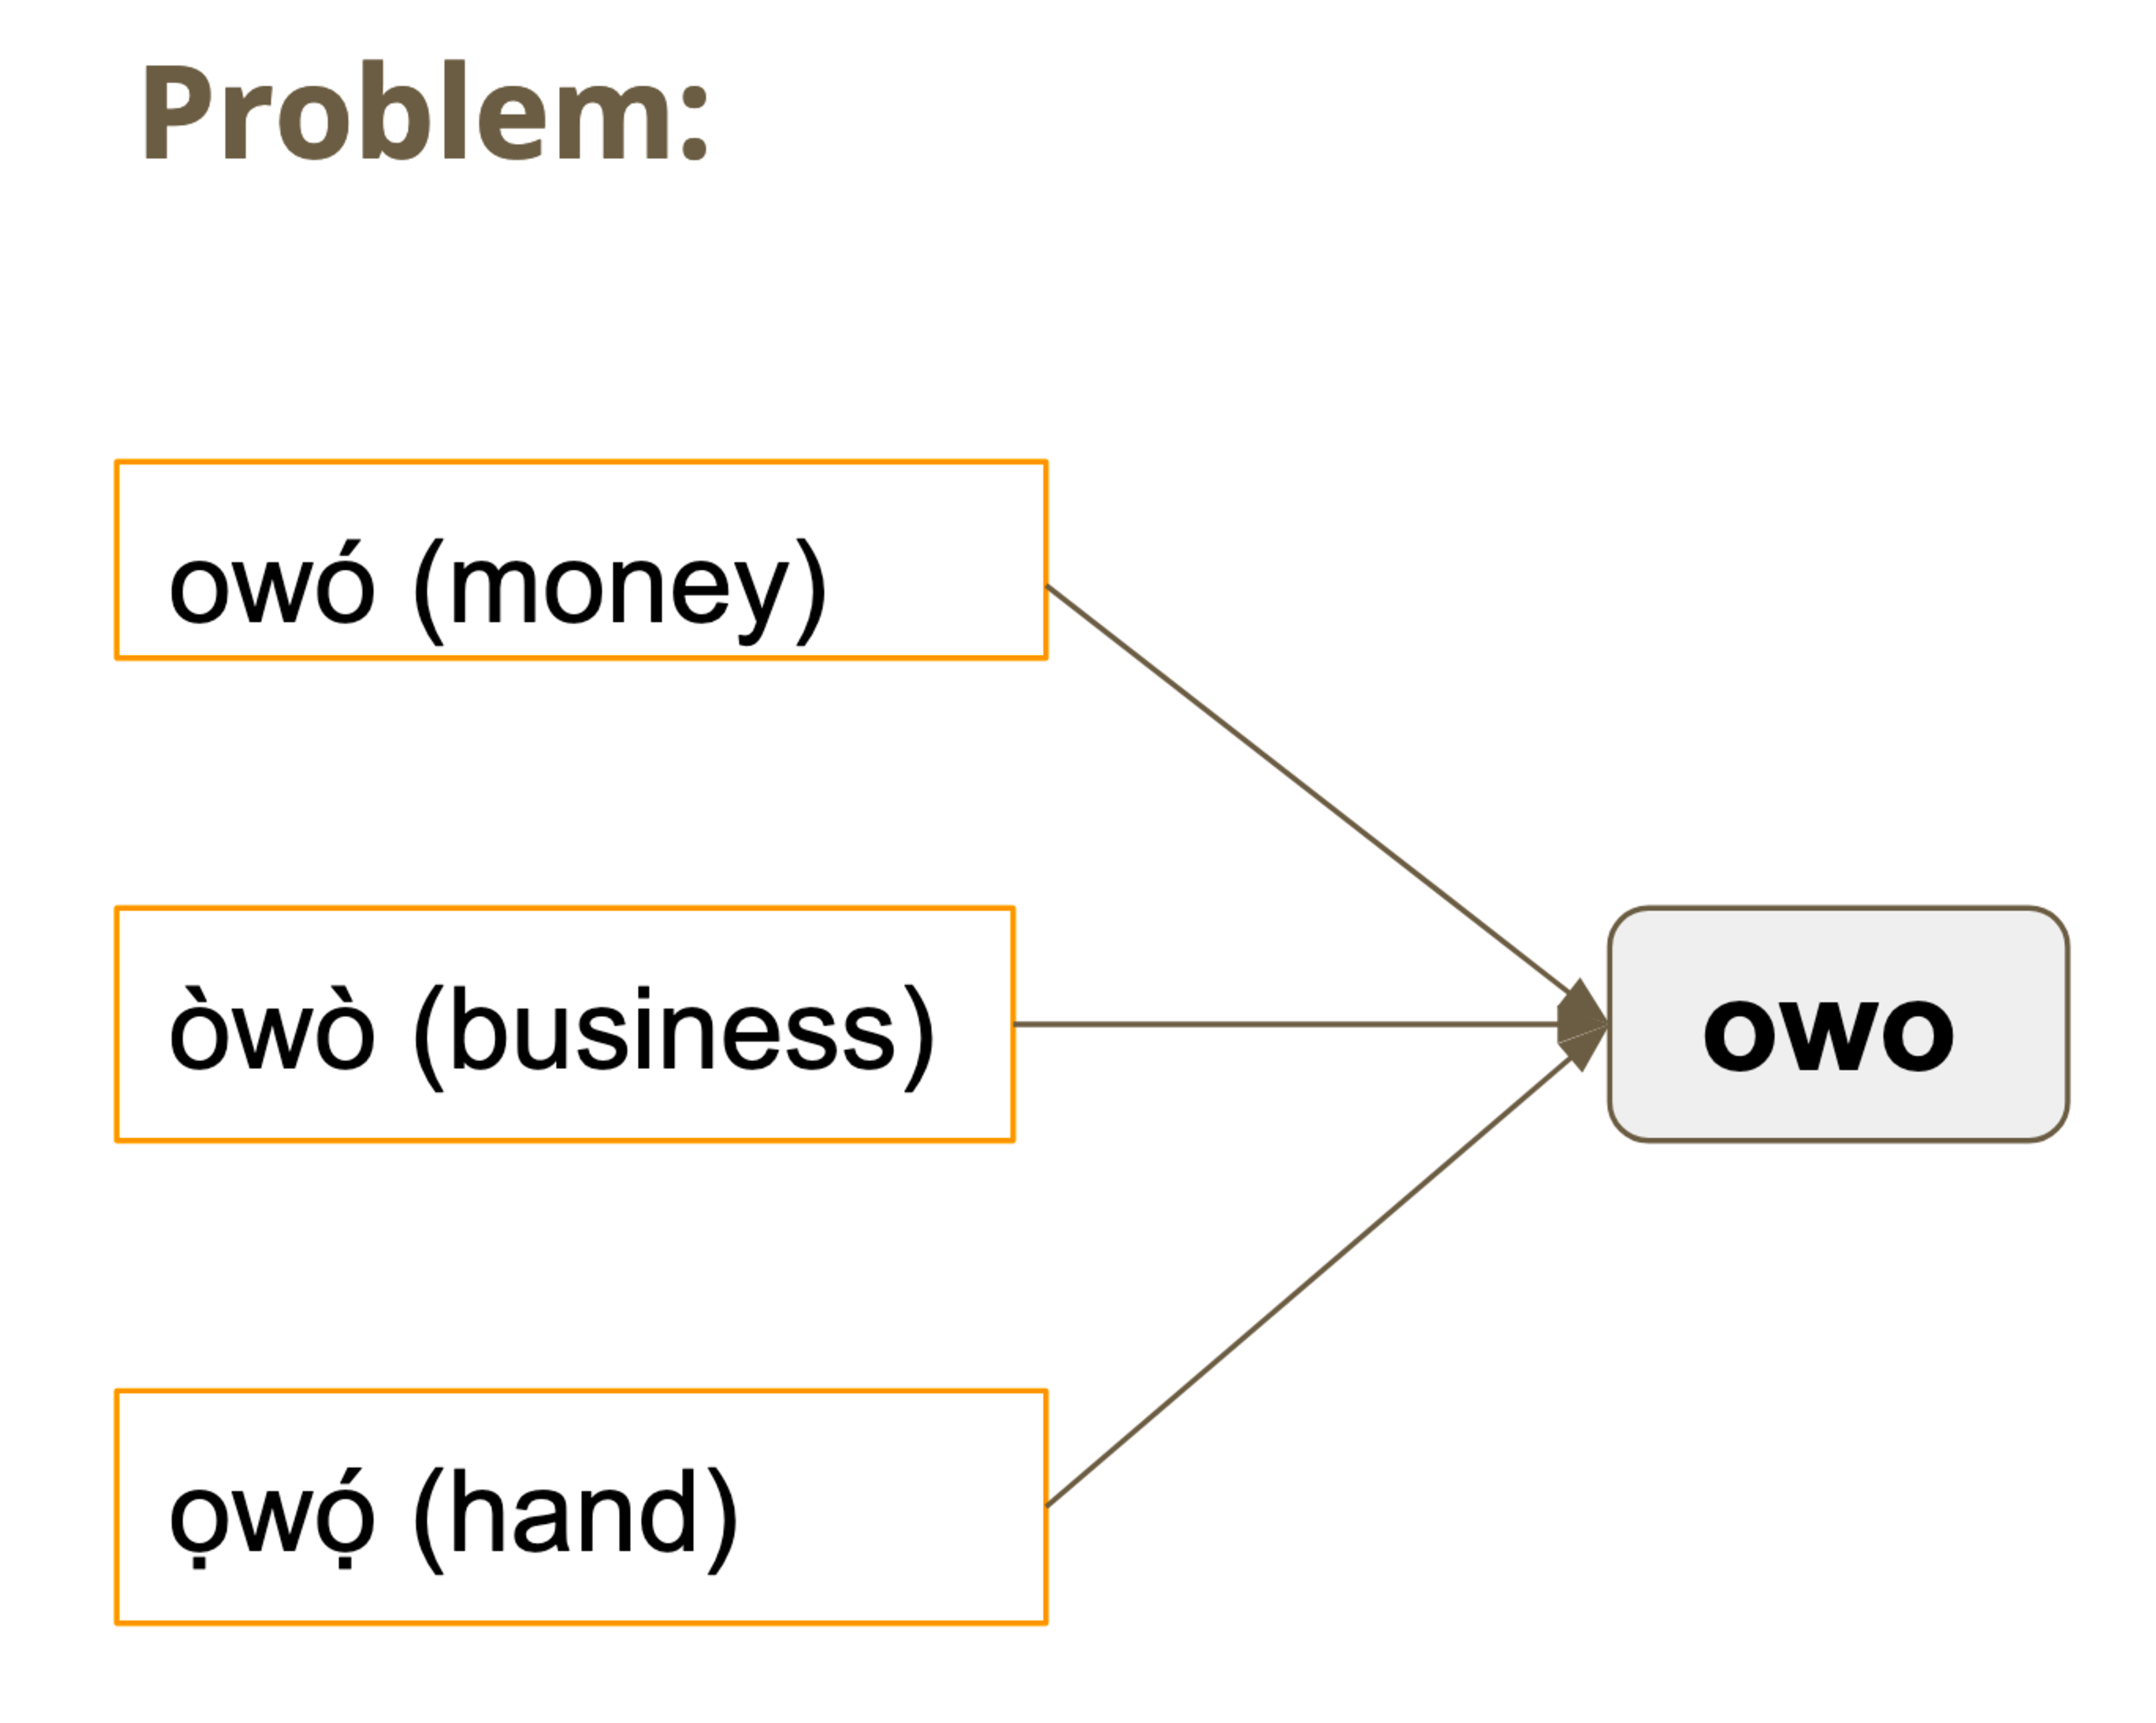
\includegraphics[trim = 0mm 0mm 0mm 0mm, clip, width=0.80\textwidth]{figures/problem.pdf}
\end{center}

\vspace{5mm}
Automatic diacritic restoration (ADR) systems facilitate text entry and correction that promotes the correct orthography and quotidian usage of the language in electronic media.

\end{block}

\vspace{5mm}

\end{column} % End of the first column

\begin{column}{\sepwid}\end{column} % Empty spacer column

\begin{column}{\onecolwid}


\begin{block}{Datasets}

\begin{center}
Data sources, prevalence and category of text

 \begin{table}[h]
  \label{tab:training_datasets}
  \begin{center}
  \begin{tabular}{rll}
    \toprule
    \textbf{\# words} & \textbf{Source}  & \textbf{Description} \\
    \midrule
    24,868 & rma.nwu.ac.za  & Lagos-NWU corpus \\  
    50,202 & theyorubablog.com & language blog \\ 
    910,401 & bible.com/versions/911 & Biblica (NIV) \\
    \midrule
    11,488,825 & opus.nlpl.eu & JW300 \\
    831,820 & bible.com/versions/207 & KJV \\
    177,675 & GitHub & Embeddings dataset \\
    142,991 & GitHub & Language ID corpus \\
    47,195 &  & Yor{\`u}b{\'a} lexicon \\
    29,338 & yoruba.unl.edu & Proverbs \\
    2,887 & unicode.org/udhr & Human rights edict \\
    \midrule
    150,360 & Private sources & Conversations \\
    15,281 & Private sources & Short stories \\
    20,038 & OCR & H{\'a}{\`a} {\`E}n{\`i}y{\`a}n (Fiction) \\
    \midrule
    \midrule
    28,308 & yo.globalvoices.org & Global Voices news \\
    \bottomrule
  \end{tabular} 
  \end{center}
\end{table}

  \end{center}
\end{block}


\vspace{15mm}

\begin{block}{Approach}

\begin{center}
% \includegraphics[trim=left bottom right top, clip]{file}
  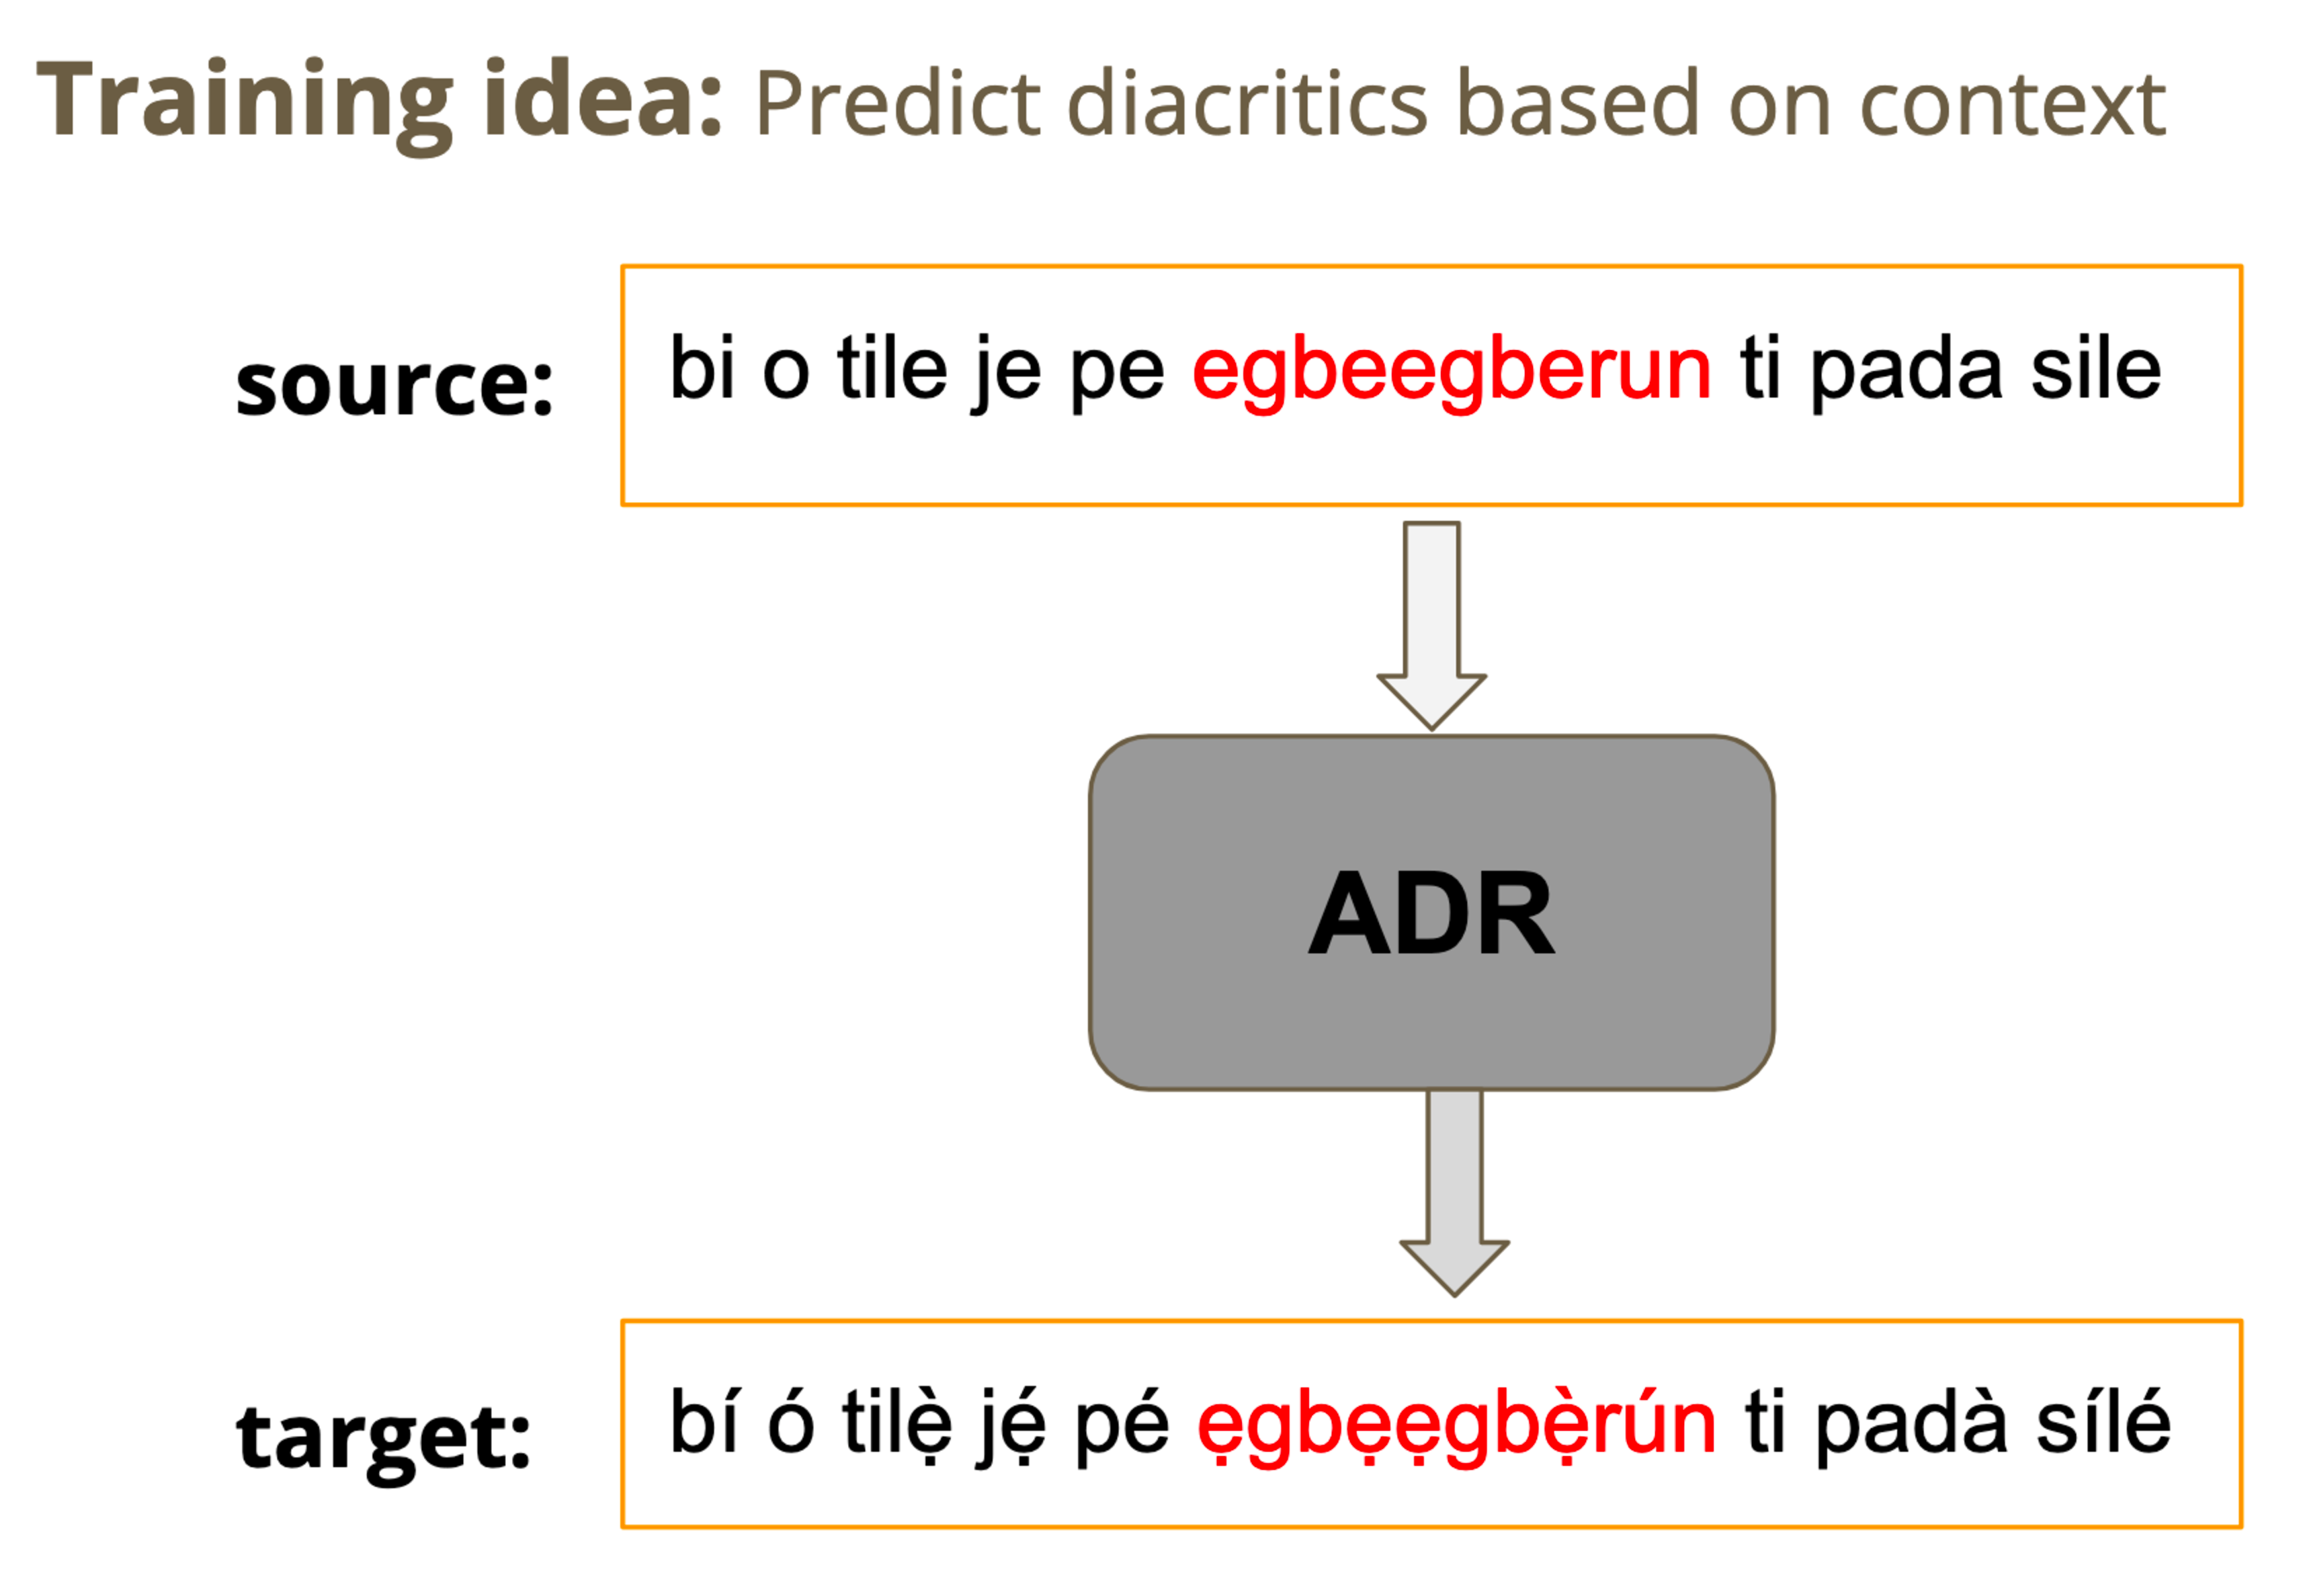
\includegraphics[trim = 0mm 0mm 0mm 0mm, clip, width=1.0\textwidth]{figures/training.pdf}
\end{center}

\end{block}

\end{column} % End of the second column

% % % % % % % % % % % % 


\begin{column}{\sepwid}\end{column} % Empty spacer column
\begin{column}{\twocolwid} % The third column

\begin{block}{This Work}

\begin{center}
% \includegraphics[trim=left bottom right top, clip]{file}
%  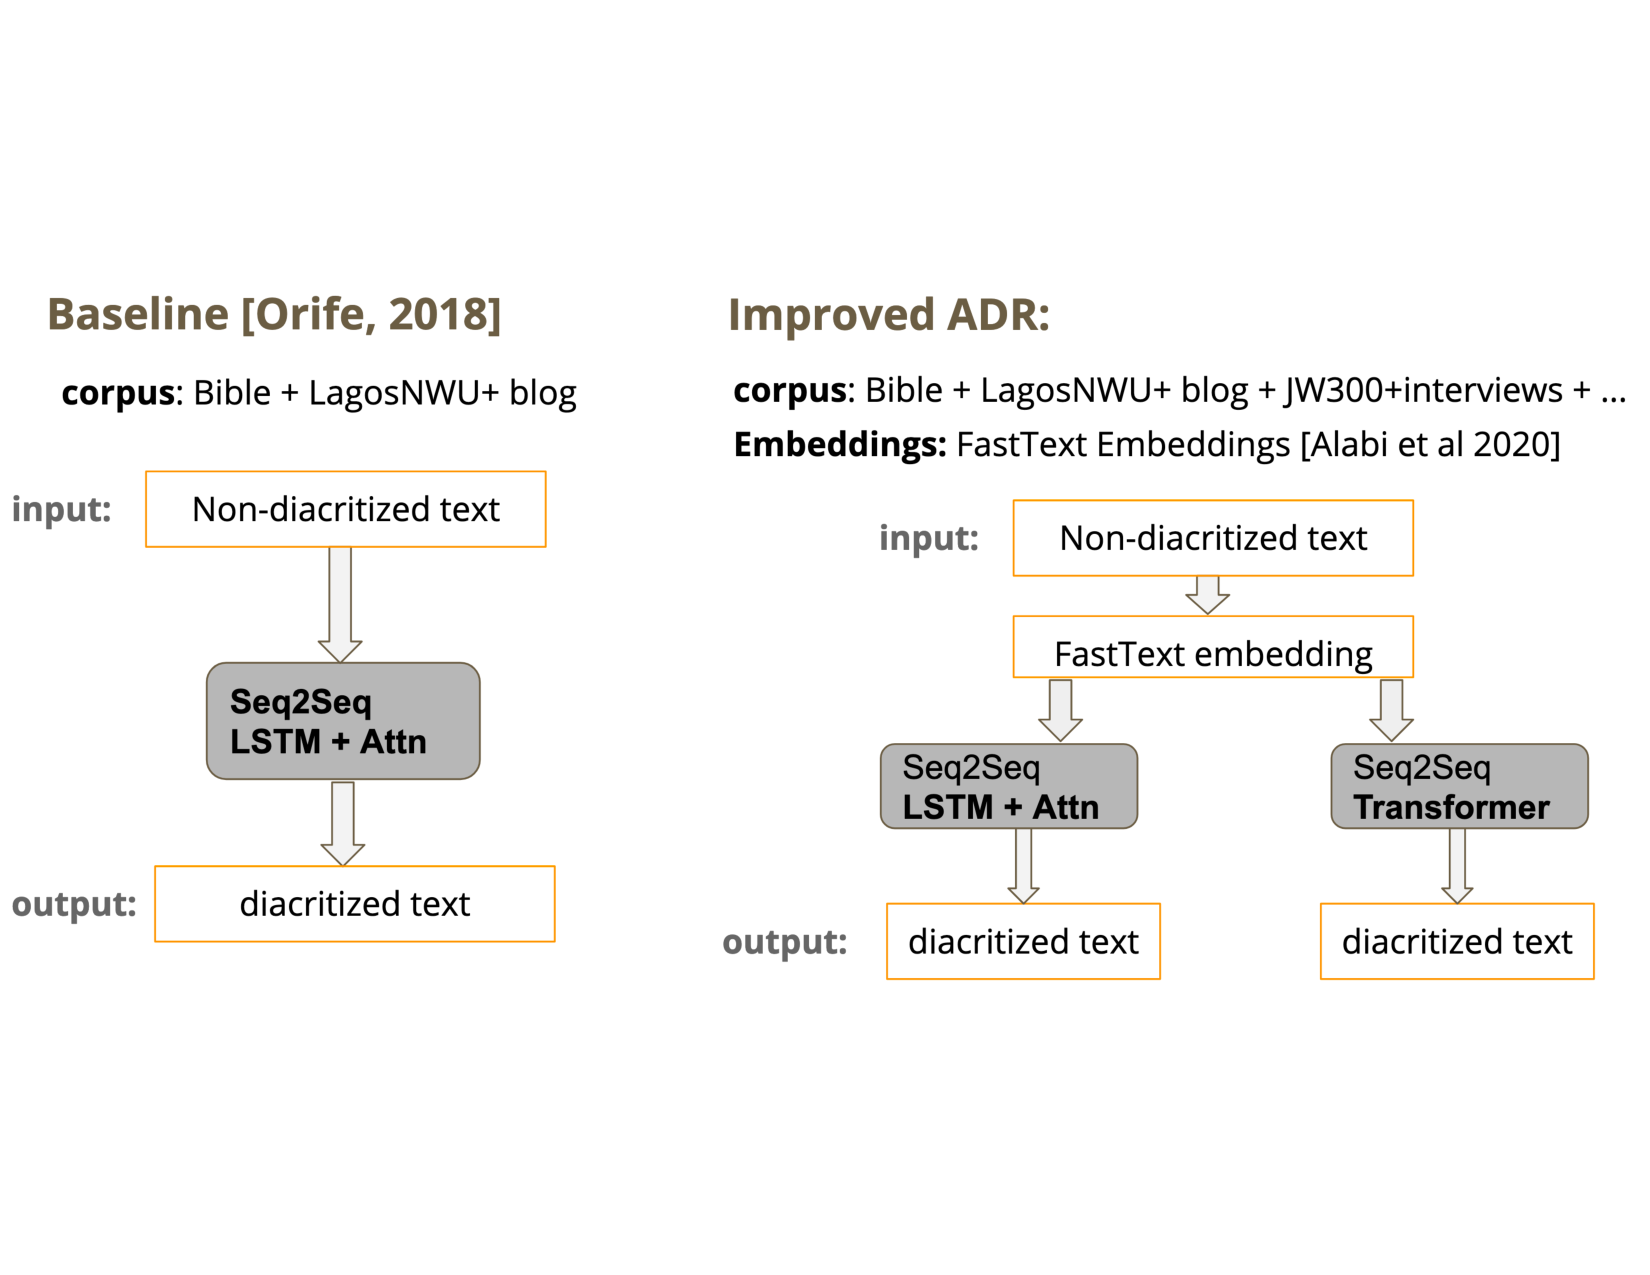
\includegraphics[trim = 0mm 60mm 0mm 55mm, clip, width=0.8\textwidth]{figures/improving.pdf}
  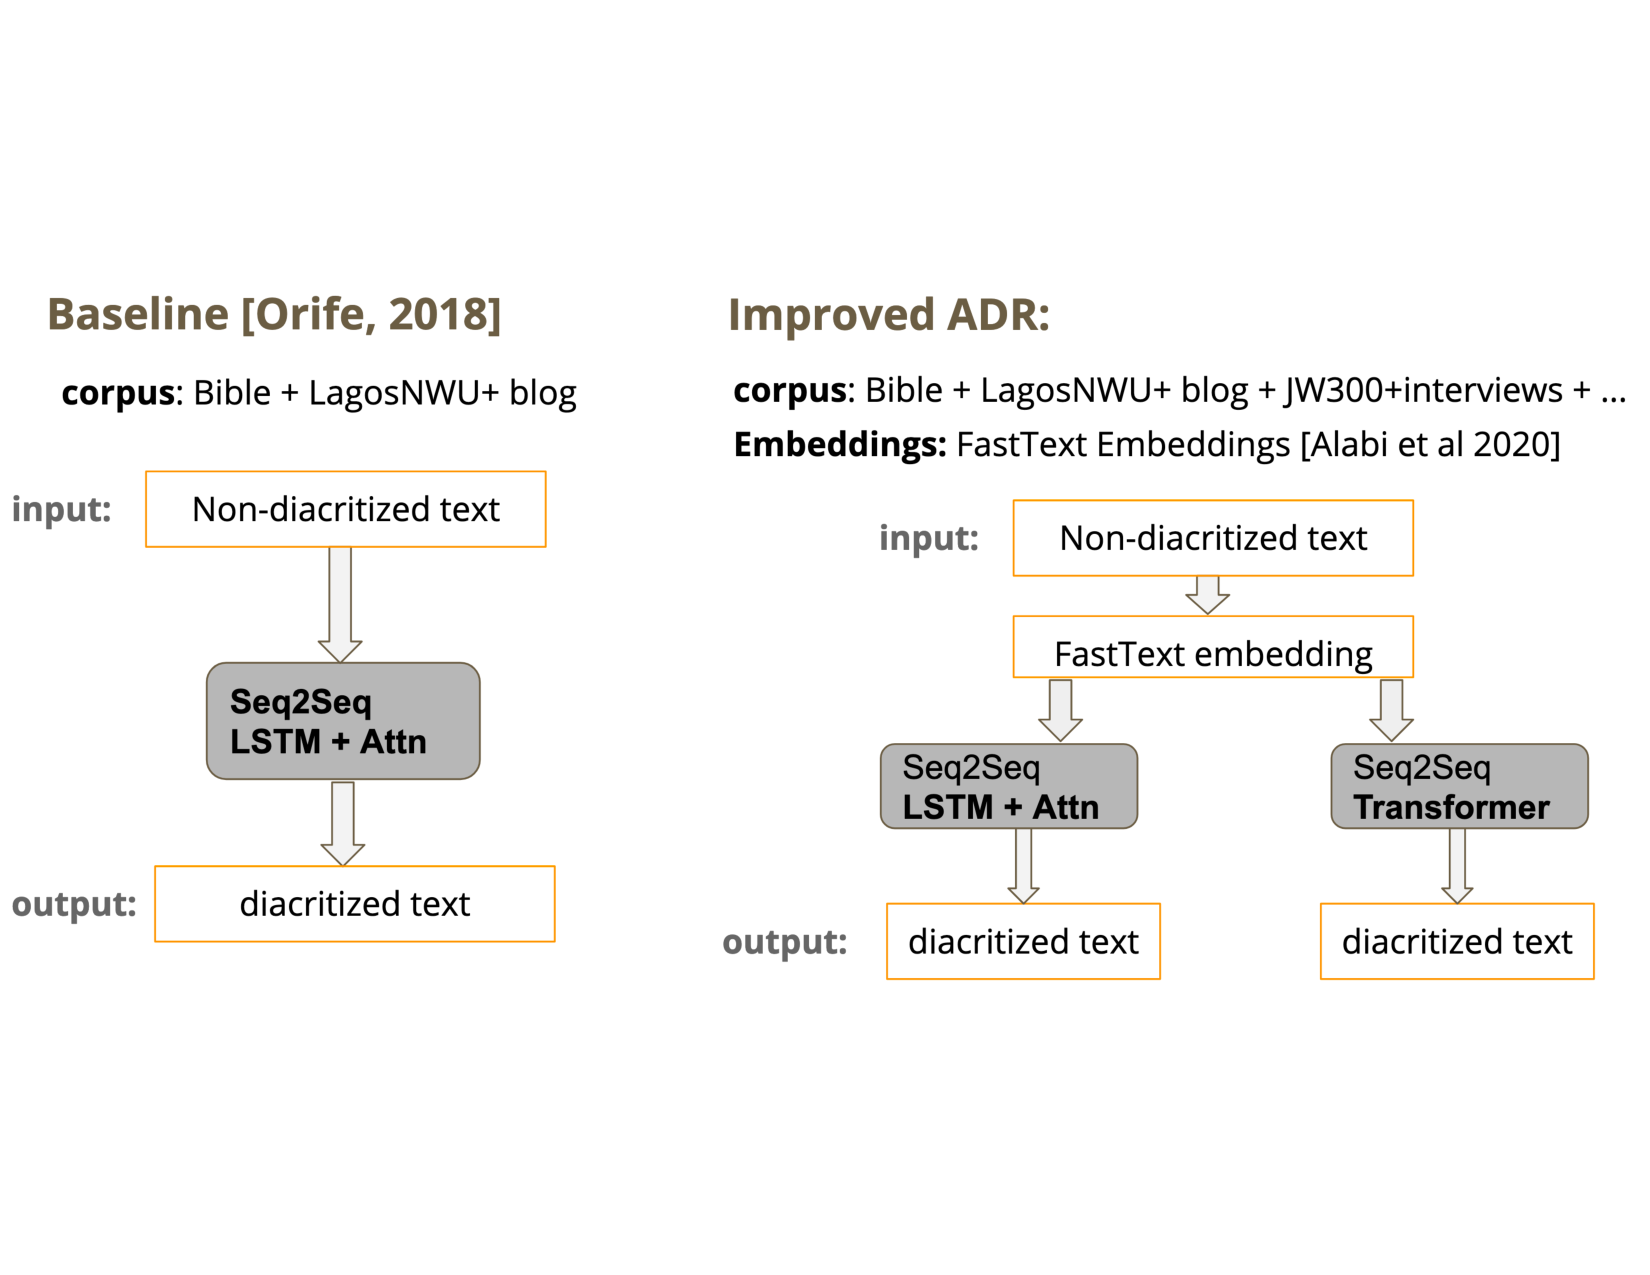
\includegraphics[trim = 0mm 50mm 0mm 45mm, clip, width=0.7\textwidth]{figures/improving.pdf}

\end{center}
\end{block}

% % % % % % % % % % % % 


\begin{columns}[t,totalwidth=\twocolwid] % Split up the two columns wide column again

\begin{column}{\twocolwid} % The first column within column 2 (column 2.1)
\begin{block}{Results}

\begin{center}
BLEU scores, predicted perplexity \& WER on the Global Voices testset

% \includegraphics[trim=left bottom right top, clip]{file}
  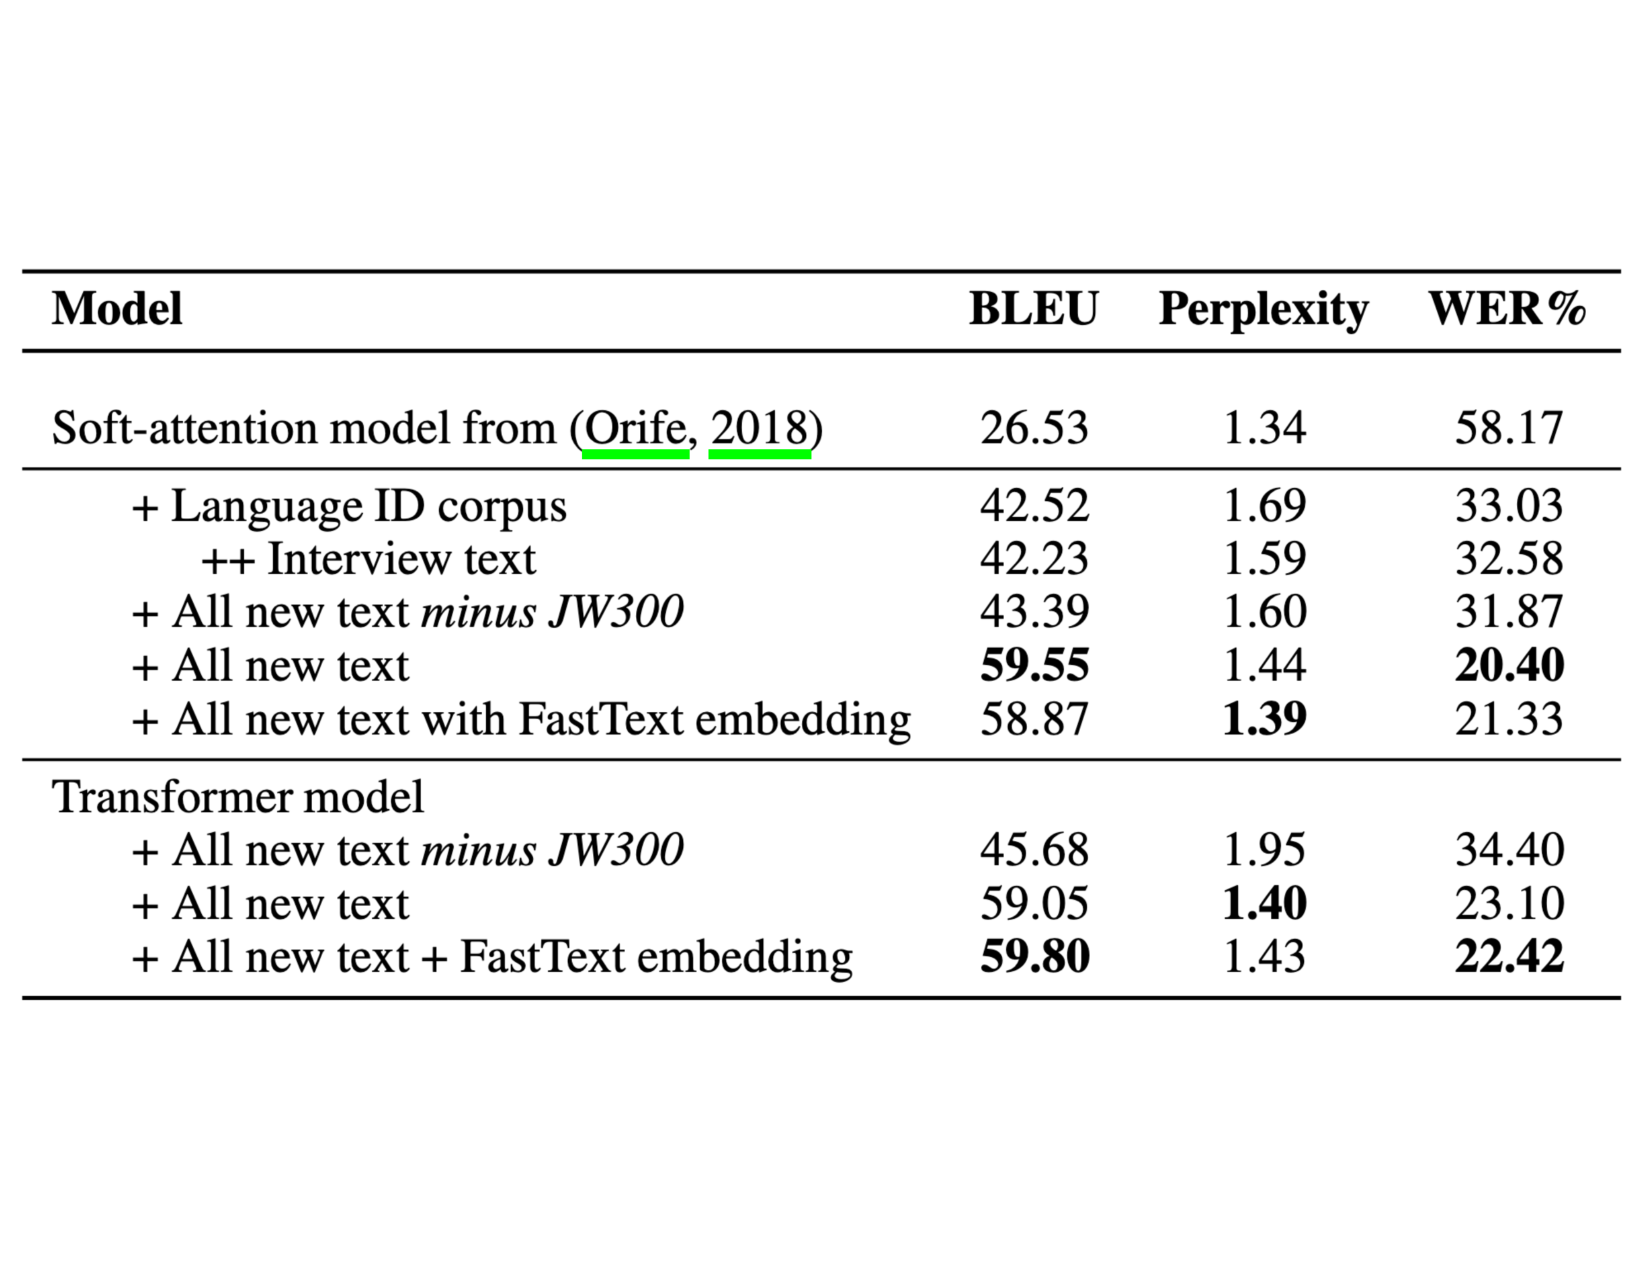
\includegraphics[trim = 0mm 50mm 0mm 35mm, clip, width=0.80\textwidth]{figures/results.pdf}
\end{center}

\end{block}

%----------------------------------------------------------------------------------------

\end{column} % End of column 2.1



%\begin{column}{\onecolwid} % The second column within column 2 (column 2.2)
%
%\begin{block}{References}
%
%% {\small
%% [Lazaridou et al., 2016] Lazaridou, Angeliki and Peysakhovich, Alexander and Baroni, Marco (2016). \\
%% Multi-agent cooperation and the emergence of (natural) language. \\
%% \href{https://arxiv.org/abs/1612.07182}{In Proceedings of ICLR}
%
%% \vspace{5mm}
%
%% [Jorge et al., 2016] Jorge, Emilio and K{\aa}geb{\"a}ck, Mikael and Gustavsson, Emil (2016). \\
%% Learning to Play Guess Who? and Inventing a Grounded Language as a Consequence. \\
%% \href{https://arxiv.org/abs/1611.03218}{arXiv preprint arXiv:1611.03218}
%% }
%
%\nocite{*} % Insert publications even if they are not cited in the poster
%\footnotesize{\bibliographystyle{apalike}
%\bibliography{main}\vspace{0.75in}}
%
%\end{block}
%
%\end{column} % End of column 2.2

\end{columns} % End of the split of column 2



\end{column} % End of the third column

\end{columns} % End of all the columns in the poster

\end{frame} % End of the enclosing frame

\end{document}
